\documentclass{beamer}
 
% === DATA === (((
\title{\sc Ejercicio 13--4 \\ M. Spivak. Caluclus.}
\author{Por Erick I. Rodríguez Juárez.}
\institute{VALUAMI}
\date{Miércoles, 7 de Agosto, 2024.}
% )))

% === FONT === (((
% \setbeamerfont{normal text}{series= \ttfamily}
% \AtBeginDocument{\usebeamerfont{normal text}}
\usefonttheme{professionalfonts}
\usefonttheme{serif}
\usepackage{fontspec}
\setmainfont[
  BoldFont       = bodonibi,
	ItalicFont     = Century modern italic2.ttf,
	BoldItalicFont = bodonibi,
	SmallCapsFont  = lmromancaps10-regular.otf
]{Century_modern.ttf}
% )))

% === FONT IN MATH MODE === (((
\DeclareSymbolFont{italics}{\encodingdefault}{\rmdefault}{m}{it}
\DeclareSymbolFontAlphabet{\mathit}{italics}
\ExplSyntaxOn
\int_step_inline:nnnn { `A } { 1 } { `Z }
 {  \exp_args:Nf \DeclareMathSymbol{\char_generate:nn{#1}{11}}{\mathalpha}{italics}{#1} }
\int_step_inline:nnnn { `a } { 1 } { `z } {  \exp_args:Nf \DeclareMathSymbol{\char_generate:nn{#1}{11}}{\mathalpha}{italics}{#1}}
\ExplSyntaxOff
% )))

% === COMMANDS === (((
\hfuzz=5pt % size of boxes
\newcommand{\dis}{\displaystyle}
\renewcommand{\qed}{\hspace{0.5cm}\rule{0.16cm}{0.4cm}}
\newcommand{\operator}[1]{\mathop{\vphantom{\sum}\mathchoice
{\vcenter{\hbox{\huge $#1$}}}
{\vcenter{\hbox{\Large $#1$}}}{#1}{#1}}\displaylimits}
\newcommand{\suma}{\operator{
\includegraphics[scale=0.09]{IMAGES/PORTADA/Sigma.png}}}
% )))

% === BEAMER TEMPLATE === (((
% DESPLIEGUE EN VARIAS DIAPOSITIVAS.
% display un item a la vez
\beamerdefaultoverlayspecification{<+(1)->}
% TITULOS EN SMALL CAPS
\setbeamerfont{title}{family=\scshape\huge}
\setbeamerfont{frametitle}{family=\scshape\LARGE}
\setbeamerfont{section in head/foot}{size = \normalsize, family=\scshape}

% sin footline
\setbeamertemplate{footline}{}

% \setbeamerfont{block title}{series=\sc}
% \setbeamerfont{block body}{series=\ttfamily }
% enumerates sin shade
\setbeamertemplate{enumerate items}[circle] % esto lo estoy usando para los simbolos de enumeración.
\setbeamertemplate{itemize items}[circle] % esto lo estoy usando para los simbolos de itemize.
\setbeamertemplate{section in toc}[circle] % esto lo estoy usando para los simbolos de enumeración.

% quitar espacio
% \addtobeamertemplate{titleframe}{}{\vspace{-5mm}}
% \addtobeamertemplate{block begin}{\vskip - \bigskipamount}{}
% \addtobeamertemplate{block end}{}{\vskip - \smallskipamount}
% \addtobeamertemplate{block example begin}{\vskip - \bigskipamount}{}
% \addtobeamertemplate{block example end}{}{\vskip - \smallskipamount}
% \addtobeamertemplate{block definition begin}{\vskip - \bigskipamount}{}
% \addtobeamertemplate{block definition end}{}{\vskip - \smallskipamount}

% PARA VER SECCIONES HORIZONTALMENTE
\setbeamertemplate{headline}{
\leavevmode
\hbox{
\begin{beamercolorbox}[wd=1.02\paperwidth,ht=4ex,dp=2ex]{palette quaternary}
\insertsectionnavigationhorizontal{\paperwidth}{\hskip 0pt plus1filll}{\hskip 0pt plus1filll}
\end{beamercolorbox}
}
}
% SECCIONES EN PÁGINAS.
\setbeamerfont{section title}{parent=title}
\setbeamertemplate{section page}
{
    \begin{centering}
	    \begin{beamercolorbox}[wd= \linewidth ,sep=12pt,center]{secciones}
    \usebeamerfont{frametitle}\insertsection\par
    \end{beamercolorbox}
    \end{centering}
}
\AtBeginSection{\frame{\sectionpage}}
% NUMBERS IN BIBLIOGRAPHY.
% \setbeamertemplate{bibliography item}[text]
% )))

% === COLORS === (((
\beamertemplatenavigationsymbolsempty % for remove the nav. symb.
\mode<presentation>

\colorlet{maincolor}{purple}
\colorlet{titlecolor}{teal}

\setbeamercolor{alerted text}{parent=palette secondary, bg=green!50}
\setbeamercolor*{palette primary}{   fg=white     , bg=maincolor}
\setbeamercolor*{palette secondary}{ fg=black     , bg=titlecolor!40}
\setbeamercolor*{palette tertiary}{  fg=white , bg=}
\setbeamercolor*{palette quaternary}{fg=white     , bg=black!20!maincolor}

\setbeamercolor*{titlelike}{parent=palette tertiary}
\setbeamercolor{frametitle}{parent=palette primary}

\setbeamercolor*{separation line}{}
\setbeamercolor*{fine separation line}{}
\setbeamercolor{block body}{parent=normal text,use=block title,bg=titlecolor!15!white,fg=black}
\setbeamercolor{block title}{bg=titlecolor!90!blue,fg=white}

\setbeamercolor{block title example}{bg=maincolor!80!black,fg=white}
\setbeamercolor{block body example}{bg=maincolor!15!white,fg=black}
\setbeamercolor{item projected}{bg=maincolor}

\setbeamercolor{section title}{parent=titlelike}
\setbeamercolor{secciones}{fg=black,bg=titlecolor!20}
\setbeamercolor{section in head}{parent=palette quaternary}
\setbeamertemplate{section in head/foot shaded}{\color{black!70!maincolor}\usebeamertemplate{section in head/foot}}
\mode<all>
% )))

% === TITLEPAGE === (((
\setbeamercolor{author}{fg = white}
\setbeamercolor{institute}{fg = white}
\setbeamercolor{date}{fg = white}
\newcommand{\portada}{
{
\addfontfeature{LetterSpace=-5}
\usebackgroundtemplate{
\includegraphics[width=  \paperwidth]{IMAGES/PORTADA/purple_teal.pdf}}
\begin{frame}[plain]
\titlepage
\end{frame}
}
}
% )))

\begin{document}

% === PORTADA === (((
\portada
\begin{frame}[plain,t]
	\frametitle{\centerline{Contenido.}}
	\vfill 
	\begin{minipage}[t]{0.5\linewidth}
		\setlength{\parskip}{2ex}
		\tableofcontents[part=0,sections={1-2}]
		\tableofcontents[part=1,sections={1-2}]
	\end{minipage}
	\hspace{5mm}
	\begin{minipage}[t]{0.4\linewidth}
		\setlength{\parskip}{2ex}
		\tableofcontents[part=1,sections={3-4}]
		\tableofcontents[part=2]
	\end{minipage}
	\vfill 
\end{frame}
% )))

\section[1. Introducción.]{Introducción} % (((

\subsection{Ideas Generales.} % (((
\begin{frame}[t,fragile]
	\frametitle{\subsecname}
	\begin{definition}
		Un activo es un \underline{bien} o \underline{servicio} que se posee.
	\end{definition}
	\begin{columns}[t]
		\column{0.6\textwidth}
		\vfill 
		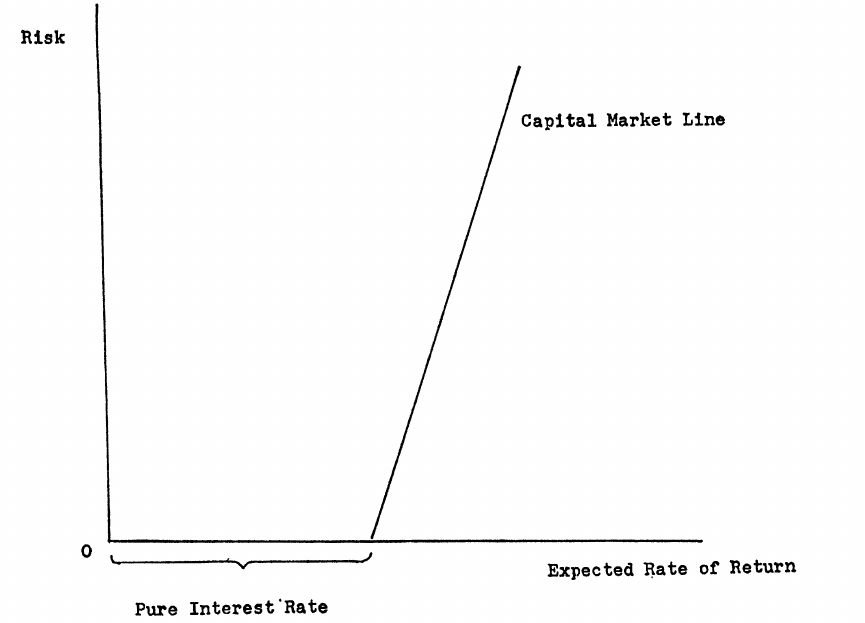
\includegraphics[width= \linewidth]{IMAGES/1/1}
		\hspace{5mm}
		\column{0.35\textwidth}
		\begin{block}{\centering Modelo Básico:}
			\begin{itemize}
				\item Precio del tiempo (Interés Puro).
				\item Precio del riesgo.
			\end{itemize}
		\end{block}
		\begin{alertblock}{\centering Supuesto:}
			Relaciones acordadas entre individuos.
		\end{alertblock}
	\end{columns}
\end{frame}

\begin{frame}[t,fragile]
	\frametitle{\subsecname}
	\begin{columns}[t]
		\column{0.6\textwidth}
		\vfill 
		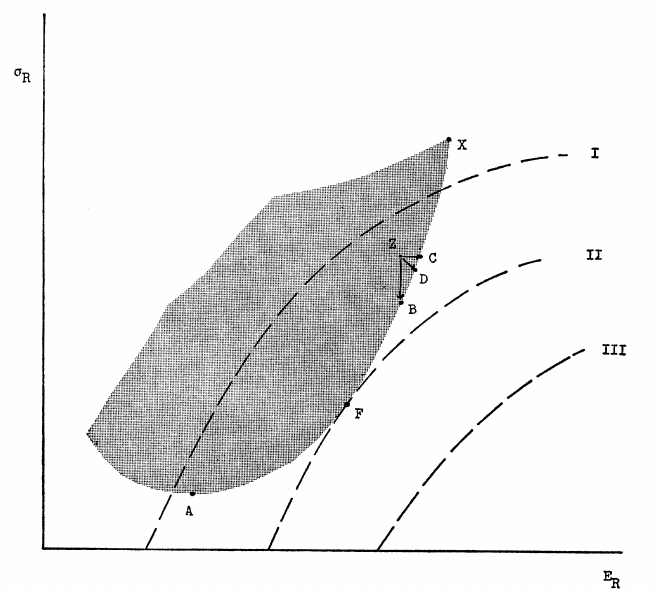
\includegraphics[width=  \linewidth]{IMAGES/1/2}
		\hspace{5mm}
		\column{0.35\textwidth}
		\begin{block}{\centering Propuesta \([\)\cite{sharpe}\(]\):}
		Hacer que la función de utilidad dependa de:
		\begin{itemize}
			\item \(E(W)\),
			\item \(\sigma (W)\).
		\end{itemize}
		\pause
		Es decir, sea de la forma:
		\[
			U = f(E_W, \sigma _W).
		\]
		Con \(f: \mathbb{R} ^2 \longrightarrow \mathbb{R}\).
	\end{block}
	\end{columns}
\end{frame}

\begin{frame}[t,fragile]
	\frametitle{\subsecname}
	\begin{block}{\centering Última simplificación:}
		Se \underline{supone} al inicio del análisis, que el inversor,
		ya ha dado una cantidad \(W_0\) al activo. \\[2mm]
		\pause
		Supongamos que después de una cantidad fija \(T\) de tiempo
		(fija para cualquier inversión), devuelve una cantidad terminal \(W_T\),
		al inversionista. \\[2mm]
		\pause
		Por tanto, la taza de regreso es:
		\[
			R_W = \dfrac{W_T - W_0}{W_0}.
		\]
		\pause
		Es decir, \(W_T = RW_0 + W_0\). \\ 
	\end{block}
\end{frame}

\begin{frame}[t,fragile]
	\frametitle{\subsecname}
	\begin{block}{\centering }
		Así, ver a \(W_T\) como variable aleatoria es equivalente a ver 
		\[
			R_W
		\]
		como variable aleatoria. \\ 
		El artículo trabaja sobre \(R\) vista como variable aleatoria y
		\[
			U = g(E_R, \sigma _R).
		\]
	\end{block}
\end{frame}
% )))

\subsection{Definiciones.} % (((
\begin{frame}[t,fragile]
	\frametitle{\subsecname}
	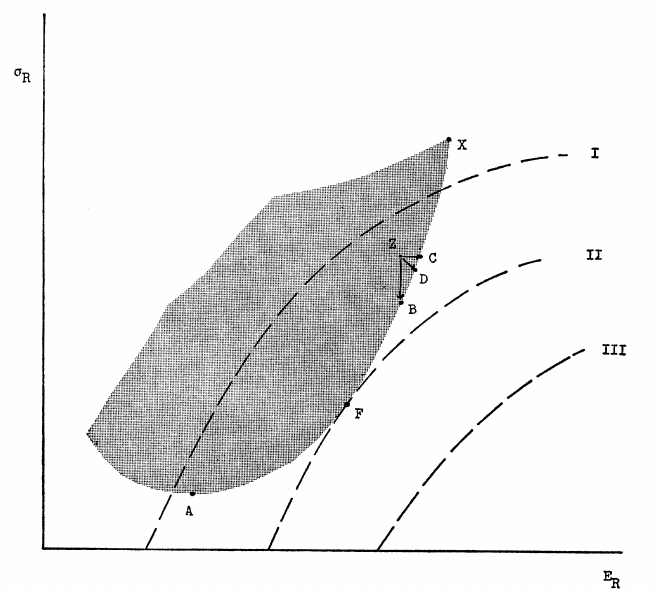
\includegraphics[width= 0.75 \linewidth, page = 1]{IMAGES/1/2}
\end{frame}

\begin{frame}[t,fragile]
	\frametitle{\subsecname}
	\begin{definition}
		Sea \((\Omega , \Sigma , P)\) espacio de probablidad \\
		\pause
		Decimos que \(X: \Omega \longrightarrow \mathbb{R}\) es medible si
		\[
			\forall a \in \mathbb{R} , \hspace{1cm} 
			X^ {-1} ((- \infty ,a]) \in \Sigma.
		\]
		\pause
		Definimos
		\(Med(\Omega) = 
		\{X \in \mathbb{R} ^ \Omega : X \mbox{ es medible}\}\).
	\end{definition}
	\pause
	\begin{definition}
		Sea \(\mathscr{R} \subseteq Med(\Omega)\).
	\end{definition}
	\pause
	En nuestro caso,
	\(\mathscr{R}\) representa el conjunto de opciones de inversión.
\end{frame}

\begin{frame}[t,fragile]
	\frametitle{\subsecname}
	\begin{block}{\centering Axiomas de vNM:}
		Supondremos que existen dos relaciones \(\leqslant , \sim \subseteq 
		\mathscr{R} ^ 2\) tales que se tienen las sig. propiedades:
		\begin{itemize}
			\item (Completez) \\ 
				\(\mathscr{R}\) es totalmente ordenado. \\ 
				Es decir, existe \(\leqslant \subseteq \mathscr{R} ^ 2\),
				tal que
				\[
					\forall L,M \in \mathscr{R} \;,\; 
					(L \leqslant M) \;\vee\; (M \leqslant L).
				\]
			\item (Transitividad) 
				\[
					(L \leqslant M) \;\land\; (M \leqslant N) \;\implies\; 
					(L \leqslant N).
				\]
		\end{itemize}
	\end{block}
\end{frame}

\begin{frame}[t,fragile]
	\frametitle{\subsecname}
	\begin{block}{\centering Axiomas de vNM:}
		\begin{itemize}
			\item (Indiferencia) \\ 
				\(\sim\) es relación de equivalencia. \\ 
				\(L \sim M\) se interpreta que al individuo le es 
				\textit{indiferente} seguir el
				plan \(L\) al plan \(M\).
			\item (Continuidad) \\ 
				Si \(L \leqslant M \leqslant N\), entonces \(\exists p \in [0,1]\),
				\[
					pL + (1-p) N \sim M.
				\]
			\item (Independencia) \\ 
				\(\forall L,M,N \in \mathscr{R}\), 
				\(\forall p \in [0,1)\),
				\[
					L \leqslant N \iff 
					(1-p) L + pM \leqslant (1-p) N + pM.
				\]
		\end{itemize}
	\end{block}
\end{frame}

\begin{frame}[t,fragile]
	\frametitle{\subsecname}
	\begin{theorem}[von-Neumann Morgenstern]
		Si se satisfacen los axiomas anteriores,
		\(\exists u: \mathbb{R} \longrightarrow \mathbb{R}\), tal que
		\[
			L \leqslant M \iff 
			E(u(L)) \leqslant E(u(M)).
		\]
	\end{theorem}
	\pause
	Así, se tienen ordenadas las esperanzas, y el eje \(E_R\).
\end{frame}
% )))

% )))

\addtocounter{part}{1}

\section[2. Política de Inversión Óptima.]{Política de Inversión Óptima} % (((

\subsection{Función de Preferencia del Inversor.} % (((
\begin{frame}[t,fragile]
	\frametitle{\subsecname}
	\vspace{-5mm}
	\begin{columns}[t]
		\column{0.7\textwidth}
		\vfill
		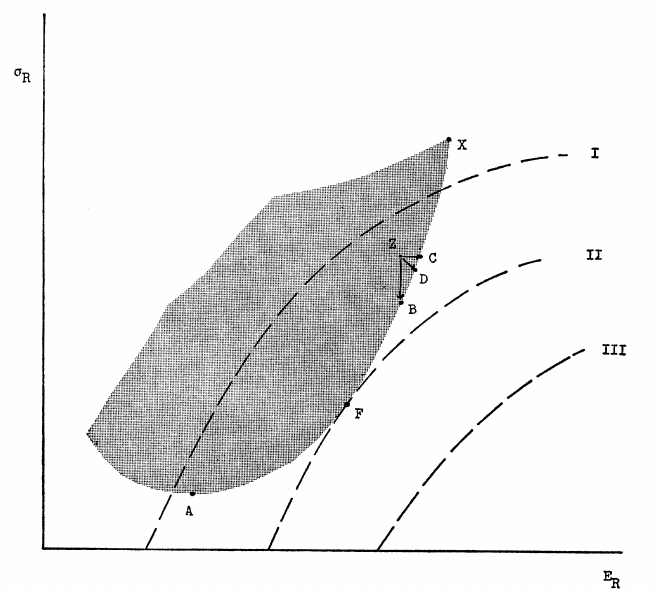
\includegraphics[width= \linewidth, page = 1]{IMAGES/1/2}
		\column{0.25\textwidth}
		\begin{block}{}
			Se espera que
			\begin{itemize}
				\item \(\dfrac{\partial U}{\partial E_W} > 0\),
				\item \(\dfrac{\partial U}{\partial \sigma _W} < 0\).
			\end{itemize}
		\end{block}
	\end{columns}
\end{frame}

\begin{frame}[t,fragile]
	\frametitle{\subsecname}
\begin{block}{\centering Justificación de las curvas de nivel:}
	Suponer que \(F: \mathbb{R} ^ 2 \longrightarrow \mathbb{R}\) 
	es diferenciable. \\ \pause
	Suponer que existe una curva diferenciable
	\(\gamma : \mathbb{R} \longrightarrow \mathbb{R} ^ 2\), \pause
	tal que 
	\[
		F \circ \gamma \equiv k,  \hspace{1cm} k \in \mathbb{R}
	\]
	\pause
	Entonces, por la Regla de la Cadena:
	\[
		\begin{array}{rcl}
			0 = Dk = D(F \circ \gamma ) \pause
			& = & DF (\gamma) \cdot \gamma ' \\[2mm]
			\pause
			& = & \nabla F (\gamma) \cdot \gamma ' \\[2mm]
			\pause 
			& = & [\partial F / \partial x \;,\; \partial F / \partial y] 
			 \cdot \begin{bmatrix}
				\gamma _1 ' \\ \gamma _2 '
			\end{bmatrix}.
		\end{array}
	\]
	\pause
	Es decir: \(\gamma(t)\) es ortogonal a \(\nabla F(\gamma (t))\),
	\(\forall t \in \mathbb{R}\).
\end{block}
\end{frame}

\begin{frame}[t,fragile]
	\frametitle{\subsecname}
	\begin{columns}[t]
		\column{0.45\textwidth}
		\vfill
		\begin{block}{\centering }
		En nuestro caso:
		\[
			\nabla U = [\partial U / \partial E_W \;,\; \partial U/\partial \sigma _W] 
		\]
		con \(\dfrac{\partial U}{\partial E_W} >0\), y 
		\(\dfrac{\partial U}{\partial \sigma _W} < 0\).
		\end{block}
		\column{0.45\textwidth}
		\only<1>{
			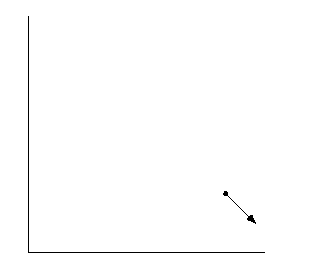
\includegraphics[width= 1.2\linewidth, page = 1]{IMAGES/2/2.pdf}
		}
		\only<2>{
			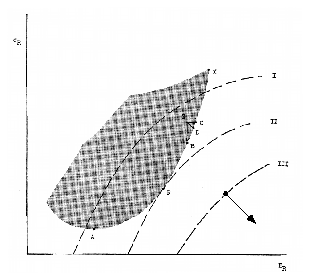
\includegraphics[width= 1.2\linewidth, page = 1]{IMAGES/3/2.pdf}
		}
	\end{columns}
\end{frame}

\begin{frame}[t,fragile]
	\frametitle{\subsecname}
	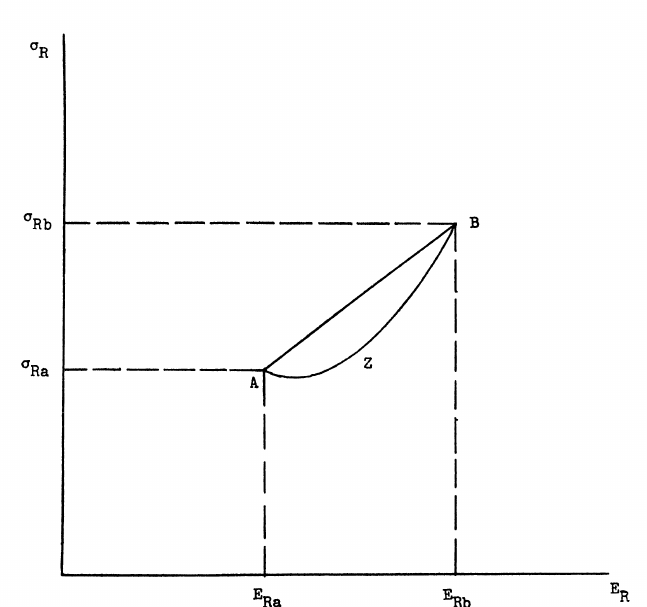
\includegraphics[width= 0.75 \linewidth, page = 1]{IMAGES/1/3}
\end{frame}

\begin{frame}[t,fragile]
	\frametitle{\subsecname}
	\begin{block}{\centering }
	Suponer que hay dos posibles inversiones \(a\) y \(b\). \\ 
	Con variables aleatorias \(R_a,R_b: \Omega \longrightarrow \mathbb{R}\). \\ 
	Queremos expresar la inversión combinada de ambos planes. \\ 
	Se define, para \(\alpha \in [0,1]\),
	\[
		R_c = \alpha R_a + (1- \alpha) R_b.
	\]
	Por tanto,
	\[
		E(R_c) = \alpha (E_a) + (1- \alpha) E(R_b).
	\]
	\end{block}
\end{frame}

\begin{frame}[t,fragile]
	\frametitle{\subsecname}
	\begin{block}{\centering }
	Además
	\[
		\begin{array}{rcl}
			var(R_c) & = & \alpha ^2 var(R_a) + (1- \alpha) ^2 var(R_b) +
			2 \cdot cov(R_a,R_b) \\[2mm]
			& = & \alpha ^2 \sigma ^ 2_a + (1- \alpha) ^2 \sigma ^2_b +
			2 \cdot \rho _{a,b} \cdot \sigma _a \sigma _b.
		\end{array}
	\]
	Puesto que \(\rho _{a,b} = \dfrac{cov(R_a,R_b)}{\sigma _a \sigma _b}\).
	Finalmente
	\[
		\sigma _c = \sqrt{\alpha ^ 2 \sigma ^ 2_a + (1- \alpha) ^ 2 \sigma ^ 2_b
		 + 2 \cdot \rho _{a,b} \cdot \sigma _a \cdot \sigma _b}.
	\]
	\end{block}
\end{frame}

\begin{frame}[t,fragile]
	\frametitle{\subsecname}
	\begin{block}{\centering}
		\textit{
			A value of \(\rho _{a,b} = 1\),
would indicate an investor's belief that there is a precise positive relation-
ship between the outcomes of the two investments.
		}
	\end{block}
	\pause
\textbf{Teorema.} \textit{Si $r(X,Y)=1$, entonces existen $m,b\in \mathbf{R}$ tales que $Y=mX+b$.}\\
\pause
\textbf{Demostración.} Definimos $f:\mathbf{R}\longrightarrow \mathbf{R}$ por $f(t)=\mathbf{E}\Big[(Y- \mathbf{E}Y)+t(X- \mathbf{E}X)\Big]^2 $, entonces 
\pause
$$\begin{array}{rcl}
  f(t)&=&\mathbf{E}(Y- \mathbf{E}Y)^2+2t\cdot  \mathbf{E}(Y- \mathbf{E}Y)(X- \mathbf{E}X)+t^2 \mathbf{E}(X- \mathbf{E}X)^2 \vspace{2mm}\\
	\pause
  &=&var(Y)+2cov(X,Y)\cdot t+var(X)\cdot t^2.
\end{array}$$
\pause
Entonces $f$ es un polinomio en $t$.
\end{frame}

\begin{frame}[t,fragile]
	\frametitle{\subsecname}
	Si $r(X,Y)=1$ (\(r^2(X,Y) = 1\)), entonces $\dfrac{cov^2(X,Y)}{var(X)\cdot var(Y)}=1$,
	\pause
$$\begin{array}{rr}
  \therefore &cov^2(X,Y)-var(X)\cdot var(Y)=0 \vspace{2mm}\\
  \therefore &\big[2cov(X,Y)\big]^2-4var(X)var(Y)=0
\end{array}$$
\pause
\textit{i.e.} el discriminante de $f$ es $0$. Y por tanto $f$ se anula una única vez en un número $a \in \mathbf{R}$, 
$$0=f(a)=\mathbf{E}\Big[(Y- \mathbf{E}Y)+a(X- \mathbf{E}X)\Big]^2 $$
\pause
Ahora, si \(U\) es variable aleatoria discreta con
	\begin{itemize}
		\item \(U \geqslant 0\),
		\item \(E(U) = 0\).
	\end{itemize}
\end{frame}

\begin{frame}[t,fragile]
	\frametitle{\subsecname}
	Por tanto, \(\forall x_i \in ImU\),
	\[
		0 \geqslant \mathbf{E}(U) = \pause
		\dis\suma_{i=0}^{n} x_iP(U=x_i) 
		\pause
		\geqslant x_iP(U = x_i) \geqslant 0.
	\]
	Entonces \(x_i \cdot P(U = x_i) =0 \;\implies\; x_i = 0 \;,\; 
	\forall x_i \in ImU\). \\ 
	\pause
	Luego \(U = 0\).
	\pause
	Hemos provado que
	\[
		\mathbf{E} \Big[(Y- \mathbb{E} Y) + a(X - \mathbb{E} X)\Big] ^ 2 = 0
	\]
	\pause
Vemos que $Y- \mathbf{E}Y+a(X- \mathbf{E}X)=0$, y en consecuencia, 
$$Y=-aX+(a \mathbf{E}X+ \mathbf{E}Y).$$
\end{frame}

\begin{frame}[t,fragile]
	\frametitle{\subsecname}
	El número \(a\) en el que se anula 
	\[
  f(t) =var(Y)+2cov(X,Y)\cdot t+var(X)\cdot t^2,
	\]
	es:
	\[
		a = \dfrac{-2 cov(X,Y) \pm \sqrt{0}}{2 var(X)}.
	\]
	Entonces \((-a) >0\), porque \(r(X,Y) =1\), indica que \(cov(X,Y) >0\).
	$$Y=-aX+(a \mathbf{E}X+ \mathbf{E}Y).$$
	La correlación lineal es positiva. \qed
\end{frame}

\begin{frame}[t,fragile]
	\frametitle{\subsecname}
	\begin{block}{\centering}
		\textit{
			A value of \(\rho _{a,b} = 0\) would
indicate a belief that the outcomes of the two investments are completely
independent}
	\end{block}
	\pause
	\textbf{Contraejemplo:} Considere una variable aleatoria discreta
	\(X : \Omega \longrightarrow \{-1,0,1\}\) sobreyectiva con
	\[
		P(X=-1) = P(X =0) = P(X = 1) = \dfrac{1}{3}.
	\]
	Considere \(Y = X ^ 2\). \\ 
	\pause
	Entonces
	\[
		\begin{array}{rcl}
		P(X = -1 , Y = 0) = \pause
			P(X = -1, X ^ 2 =0) & = &
			P(X = -1, X = 0) \\[2mm] 
		\pause
			& = & P(\varnothing) \\[2mm] 
			& = & 0.
		\end{array}
	\]
\end{frame}

\begin{frame}[t,fragile]
	\frametitle{\subsecname}
	Pero
	\[
		P(X=-1) \cdot P(Y =0) = \dfrac{1}{3} \cdot \dfrac{1}{3} \ne 
		0 = P(X=-1,Y=0).
	\]
	\pause
	Entonces \(X\) y \(Y\) no son independientes. \\[2mm]
	\pause
	Notar que
	\[
		E(X) = \dfrac{1}{3} \cdot (-1) + \dfrac{1}{3} \cdot 0 
		+ \dfrac{1}{3} \cdot 1 = 0.
	\]
	\pause
	Indicando 
	\[
		E(XY) = \pause
		E(X ^ 3) = \pause
		E(X) = \pause
		0 = \pause
		0 \cdot E(Y) = \pause
		E(X) \cdot E(Y).
	\]
	Finalmente
	\[
		r(X,Y) = cov(X,Y) / \sigma _X \sigma _Y
		\pause
		= \dfrac{E(XY) - E(X) E(Y)}{\sigma _X \sigma _Y} = 0. \qed
	\]
\end{frame}

\begin{frame}[t,fragile]
	\frametitle{\subsecname}
	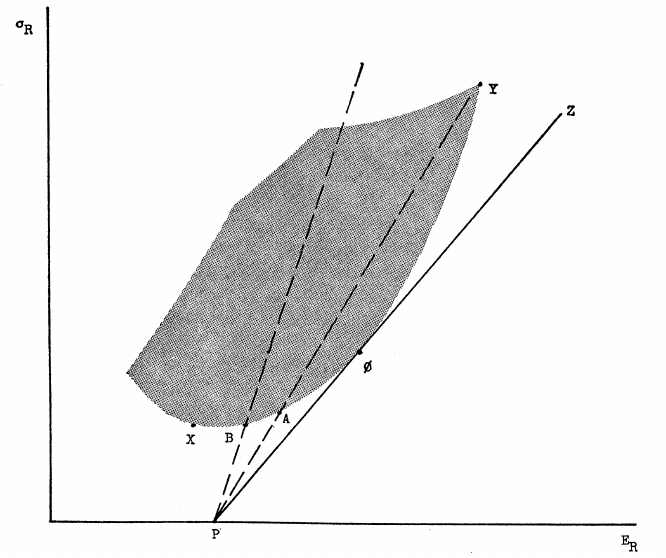
\includegraphics[width= 0.75 \linewidth, page = 1]{IMAGES/1/4}
\end{frame}

\begin{frame}[t,fragile]
	\frametitle{\subsecname}
	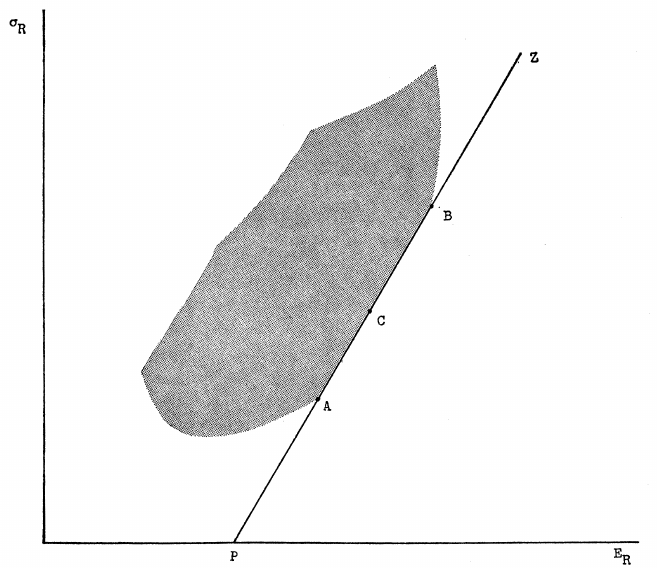
\includegraphics[width= 0.75 \linewidth, page = 1]{IMAGES/1/6}
\end{frame}
% )))

% \subsection{Curva de Oportunidad de Inversión.} % (((
% \begin{frame}[t,fragile]
	% \frametitle{\subsecname}
% \end{frame}
% )))

% \subsection{Taza de Interés Puro.} % (((
% \begin{frame}[t,fragile]
	% \frametitle{\subsecname}
% \end{frame}
% )))

% )))

% \section[3. Equil. en Merc.]{Equilibrio en Mercado de Capitales} % (((
% \begin{frame}[t]
	% \frametitle{\secname}
	% 
% \end{frame}
% )))

% \section[4. Precios de Act.]{Los Precios de Capitales Activos} % (((
% \begin{frame}[t]
	% \frametitle{\secname}
	% 
% \end{frame}
% )))

\addtocounter{part}{1}

\section[3. Conclusiones.]{Conclusiones} % (((
\begin{frame}[t,fragile]
	\frametitle{\secname}
	\begin{alertblock}{ \centering Hipótesis:}
		\begin{itemize}
			\item Continuidad (y ordenamiento) en el eje \(E_W\).
			\item Se conoce donde \(U >0\) y \(U < 0\).
			\item Zona de Riesgo.
		\end{itemize}
	\end{alertblock}
\end{frame}

\begin{frame}[t,fragile]
	\frametitle{\secname}
		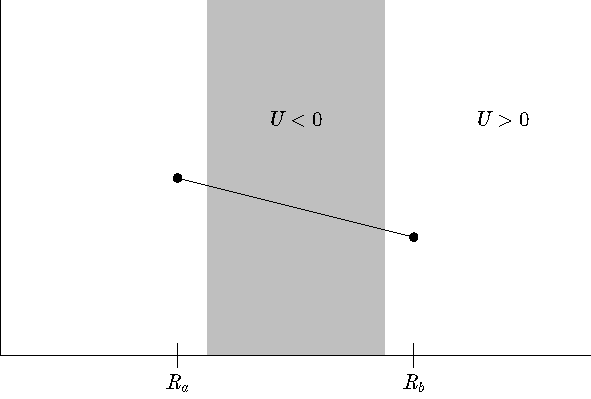
\includegraphics[width= 0.8 \linewidth]{IMAGES/4/4}
\end{frame}

\begin{frame}[t,fragile]
	\frametitle{\secname}
	\begin{alertblock}{\centering No se puede aplicar el modelo con:}
		\begin{itemize}
			\item La zona de riesgo no permite encontrarse un punto tangente.
			\item \(r_{a,b} = -1\).
		\end{itemize}
	\end{alertblock}
\end{frame}
% )))

\section{Referencias} % (((
\begin{frame}[t]
\frametitle{\secname}
\bibliography{References}
\beamerdefaultoverlayspecification{}
\bibliographystyle{unsrt}
\end{frame}
% )))

\end{document}
